\bigskip

\item The graph below could be that of

% \resizebox{3in}{!}{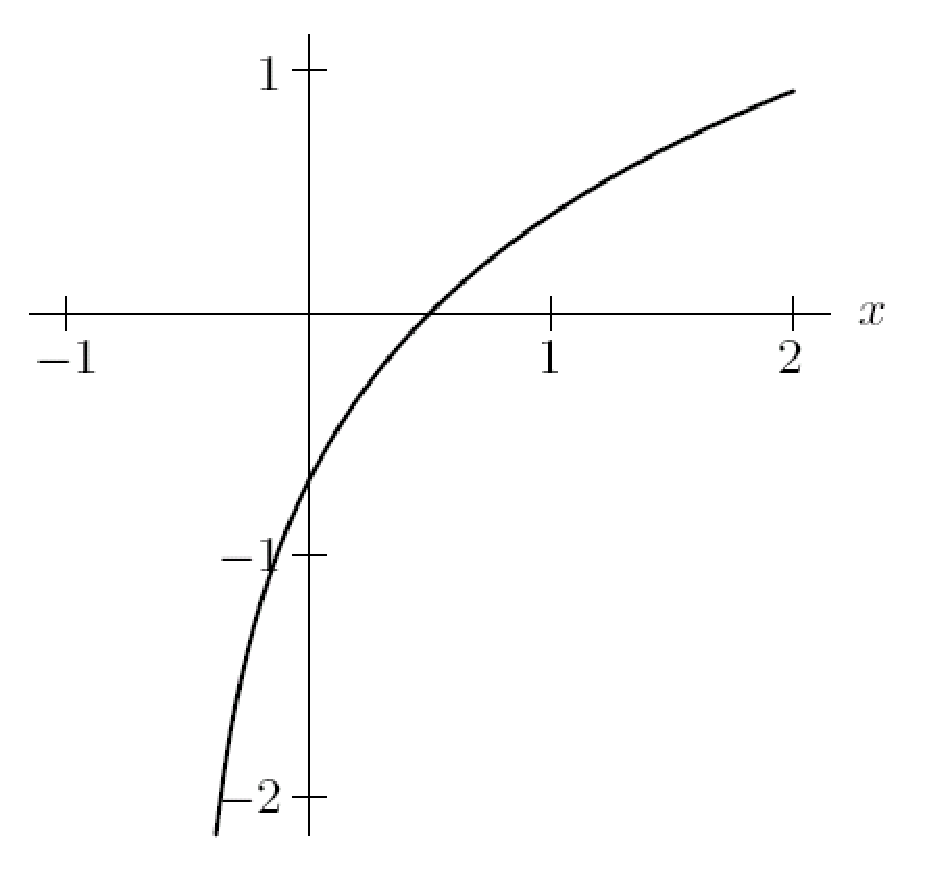
\includegraphics{SVC.01.04.020.ps}}

    \begin{minipage}{0.4\columnwidth}
        \begin{enumerate}
            \item $y = \ln x + \frac{1}{2}$
            \item $y = \ln x - \frac{1}{2}$
            \item $y = \ln \left( x + \frac{1}{2} \right)$
            \item $y = \ln \left( x - \frac{1}{2} \right)$
        \end{enumerate}
    \end{minipage}
    \begin{minipage}{0.6\columnwidth}
    \begin{center}
        \begin{tikzpicture}
            \begin{axis}[axis lines=center, xlabel={$x$}, ylabel={$y$}, xmin=-1, xmax=2,
                ymin=-3, ymax=3]
                \addplot[color=blue, very thick,domain=-1:2, samples=100] {ln(x + 0.5)};
            \end{axis}
        \end{tikzpicture}
    \end{center}
    \end{minipage}

% ConcepTests - to accompany Calculus 4th Edition, Hughes-Hallet et al. John Wiley \& Sons.
